\documentclass[12pt, twoside]{article}
\usepackage[letterpaper, margin=1in, headsep=0.2in]{geometry}
\setlength{\headheight}{0.6in}
%\usepackage[english]{babel}
\usepackage[utf8]{inputenc}
\usepackage{microtype}
\usepackage{amsmath}
\usepackage{amssymb}
%\usepackage{amsfonts}
\usepackage{siunitx} %units in math. eg 20\milli\meter
\usepackage{yhmath} % for arcs, overparenth command
\usepackage{tikz} %graphics
\usetikzlibrary{quotes, angles}
\usepackage{graphicx} %consider setting \graphicspath{{images/}}
\usepackage{parskip} %no paragraph indent
\usepackage{enumitem}
\usepackage{multicol}
\usepackage{venndiagram}

\usepackage{fancyhdr}
\pagestyle{fancy}
\fancyhf{}
\renewcommand{\headrulewidth}{0pt} % disable the underline of the header
\raggedbottom
\hfuzz=2mm %suppresses overfull box warnings

\usepackage{hyperref}

\fancyhead[LE]{\thepage}
\fancyhead[RO]{\thepage \\ Name: \hspace{4cm} \,\\}
\fancyhead[LO]{BECA / Dr. Huson / Geometry\\*  Unit 4: Volume and polyhedra \\* 1 November 2022}

\begin{document}

\subsubsection*{4.2 Classwork: Volume of a prism (box)}
\begin{enumerate}
\item Find the volume of a rectangular prism with length 5 cm, width 4 cm, and height 3 cm. \vspace{1cm}

\item A triangle has an area of 68 square centimeters. Its height is 16 centimeters. Find the length of its base. \vspace{3cm}

\item The perimeter of a square is 10 inches. Find its area. \vspace{4cm}

\item The volume of a rectangular prism (box) is $V=72$ cubic feet. Its length is $l=6$ feet and depth of $w=3$ feet. Find its height. Start with the equation \\[0.5cm]
$V = l \times w \times h = 72$
  \begin{flushright}
    \begin{tikzpicture}[scale=1.25]
      \draw [-, thick] (0,0)--(4,0)--(4,2)--(0,2)--cycle;
      \draw [-, thick] (0,2)--(0.5,2.75)--(4.5,2.75)--(4,2);
      \draw [-, thick] (4,0)--(4.5,0.75)--(4.5,2.75);
      \node at (4.75, 1.75){$h$};
      \node at (2, -0.25){$6$};
      \node at (4.5, 0.25){$3$};
    \end{tikzpicture}
  \end{flushright}

\newpage
\item Find the volume of a rectangular prism (box). Its length is $l=10$ feet, its height $h=4$, and depth is $w=3$ feet. Start with the equation \\[0.5cm]
$V = l \times w \times h$
  \begin{flushright}
    \begin{tikzpicture}[scale=1.25]
      \draw [-, thick] (0,0)--(4,0)--(4,2)--(0,2)--cycle;
      \draw [-, thick] (0,2)--(0.5,2.75)--(4.5,2.75)--(4,2);
      \draw [-, thick] (4,0)--(4.5,0.75)--(4.5,2.75);
      \node at (4.75, 1.75){$4$};
      \node at (2, -0.25){$10$};
      \node at (4.5, 0.25){$3$};
    \end{tikzpicture}
  \end{flushright}

\item The volume of a rectangular prism (box) is $V=110$ cubic feet. Its height is $h=5$ feet and depth of $w=4$ feet. Find its length. Start with the equation \\[0.5cm]
$V = l \times w \times h = 110$
  \begin{flushright}
    \begin{tikzpicture}[scale=1.25]
      \draw [-, thick] (0,0)--(4,0)--(4,2)--(0,2)--cycle;
      \draw [-, thick] (0,2)--(0.5,2.75)--(4.5,2.75)--(4,2);
      \draw [-, thick] (4,0)--(4.5,0.75)--(4.5,2.75);
      \node at (4.75, 1.75){$5$};
      \node at (2, -0.25){$?$};
      \node at (4.5, 0.25){$4$};
    \end{tikzpicture}
  \end{flushright}

\item A rectangular prism (shown below) has a volume $V=925$ cubic feet. Calculate the area of its base and then solve for its height.
\begin{multicols}{2}
\begin{enumerate}
  \item The base measures 12.5 by 4 in feet. Find its area.
  \item Find the prism's height, $x$. \vspace{2cm}
\end{enumerate}
  \begin{flushright}
    \begin{tikzpicture}[scale=1]
      \draw [-, thick] (0,0)--(3,0)--(3,4)--(0,4)--cycle;
      \draw [-, thick] (0,4)--(0.5,4.75)--(3.5,4.75)--(3,4);
      \draw [-, thick] (3,0)--(3.5,0.75)--(3.5,4.75);
      \node at (3.75, 2.75){$x$};
      \node at (1.5, -0.25){$12.5$};
      \node at (3.5, 0.25){$4$};
    \end{tikzpicture}
  \end{flushright}
\end{multicols}

\newpage
\item Find the volume of a rectangular prism (box). Its length is $l=21$ inches, its height $h=13$ inches, and depth is $w=9$ inches. Start with the equation \\[0.5cm]
$V = l \times w \times h$
  \begin{flushright}
    \begin{tikzpicture}[scale=1.25]
      \draw [-, thick] (0,0)--(4,0)--(4,2)--(0,2)--cycle;
      \draw [-, thick] (0,2)--(0.5,2.75)--(4.5,2.75)--(4,2);
      \draw [-, thick] (4,0)--(4.5,0.75)--(4.5,2.75);
      \node at (4.75, 1.75){$13$};
      \node at (2, -0.25){$21$};
      \node at (4.5, 0.25){$9$};
    \end{tikzpicture}
  \end{flushright}

\item A rectangular prism has a square base. Its volume is $V=507$ cubic centimeters and its height is $h=12$ cm.
  \begin{multicols}{2}
    Calculate the dimensions of its base.
    \begin{flushright}
      \begin{tikzpicture}[scale=1]
        \draw [-, thick] (0,0)--(3,0)--(3,4)--(0,4)--cycle;
        \draw [-, thick] (0,4)--(0.5,4.75)--(3.5,4.75)--(3,4);
        \draw [-, thick] (3,0)--(3.5,0.75)--(3.5,4.75);
        \node at (3.75, 2.75){$12$};
        \node at (1.5, -0.25){$x$};
        \node at (3.5, 0.25){$x$};
      \end{tikzpicture}
    \end{flushright}
  \end{multicols}

\item The volume of a box (rectanglar prism) is the product of its length, width, and height.
$$V = l \times w \times h$$
Example: Find the volume of a box with a length of 8 centimeters, a depth of 4 cm, and a height of 5 cm. Show the calculation.
\begin{flushright}
  \begin{tikzpicture}[scale=1.25]
    \draw [-, thick] (0,0)--(4,0)--(4,2)--(0,2)--cycle;
    \draw [-, thick] (0,2)--(0.5,2.75)--(4.5,2.75)--(4,2);
    \draw [-, thick] (4,0)--(4.5,0.75)--(4.5,2.75);
    \node at (4.75, 1.75){$5$};
    \node at (2, -0.25){$8$};
    \node at (4.5, 0.25){$4$};
  \end{tikzpicture}
  \end{flushright} \vspace{2cm} 

\item Find the volume of a box (rectanglar prism) having a length of 12 inches, a width of 6 inches, and a height of 5 inches. Show the calculation.


\end{enumerate}
\end{document}